\section{Aula 6.1 - Códigos de linha}

O objetivo dessa vídeo aula é mostrar os diversos esquemas de codificação existentes na modulação digital da informação.
O ponto crucial para entender a distinção entre esquemas é compreender como os esquemas são classficados visto que entendendo a "lógica de classificação",
fica fácil mapear um esquema ao resultado final de uma sequência de bits passando pelo mesmo. Para facilitar a compreensão introduziremos cada categoria 1 a 1 e terminaremos
com um apanhado contrastando o uso de cada uma.

\subsection{NRZ - Não Retorno ao Zero}

Porque o nomo NRZ, o que significa não retornar a zero? Veja a imagem abaixo para tentar associar a explicação ao resultado real.

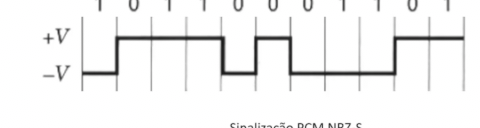
\includegraphics[width=0.6\textwidth]{../assets/nrz.png}

Bem o não retorno ao zero está no fato que o sinal elétrico de saída, o resultado da codificação, oscila sempre entre nos limites do conjunto [ +V,-V ] consequentemente nunca o bit0/1 assume o valor
de 0V, daí o nome, não retorno ao zero.

vamos agora as subidivisões que existem

\subsubsection{As possíveis subdivisões, ao que você deve estar atento?}

\textbf{L} (level) (do inglês nível): nessa subdivisão existe um mapeamento claro entre o nível lógico 0 e -V e nível lógico 1 e +V, é a figura de cima, o ponto crucial é que essa subdivisão
não é afetada pelo valor do bit anterior, não existe memória na codificação, o mapeamento é estático.
\\

\textbf{M/S} (mark/space) (do inglês marca/espaço): nessas subdivisões existe um nível lógico que alterna e outro que fica fixo e nível de tensão igual ao do que alterou, logo um nível lógico
marca a tensão usada pelo outro, efetivamente, no caso \textbf{M} é para o caso que o bit 1 é o que marca e \textbf{S} é o caso que o bit 0 é marcado.

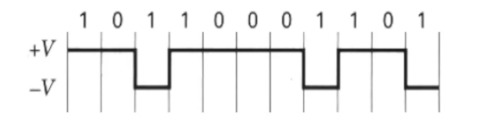
\includegraphics[width=0.6\textwidth]{../assets/nrzm.png}

\textbf{OBS:}Note que o 1 é o nível lógico que se altera nesse caso.

\textbf{OBS2:}Note que a imposição de um nível lógico ser alterado se da pelo fato que se não alterasse seria impossível distinguir os níveis lógicos visto a regra de codificação
mencionada previamente.

\subsection{RZ - Retorno ao zero}

O detalhe aqui é perceber que o nível lógico, indepedente da subdivisão, \textit{sempre retorna para o 0 por metade do intervalo de codificação de um bit}.

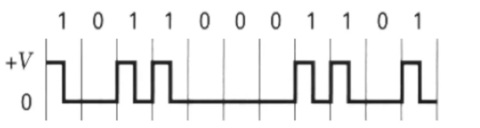
\includegraphics[width=0.6\textwidth]{../assets/rz.png}


\subsubsection{As possíveis subdivisões, ao que você deve estar atento?}

\textbf{Polar}: a distinção é clara, os níveis lógicos no final do período de transição são necessariamente +V ou -V, muito parecido com o NRZ-L, mas note que há esse retorno ao
zero que da o nome a essa família de esquemas.
\\
\\
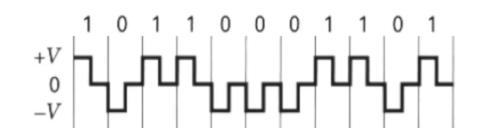
\includegraphics[width=0.6\textwidth]{../assets/polar-rz.png}
\\
\textbf{OBS:} Nesse caso é convenção que o bit 1 seja codificado por tensão positiva e o bit 0 negativa.
\\

\textbf{AMI} (Alternate mark inversion): o nome leva marca, mas note que pela representação abaixo do esquema não existe marca, visto que o bit 0 é sempre 0, infelizmente
é uma inconsistência de nomeclatura, \textbf{note que na imagem o autor não compensou o offset inicial da codificação, mas usualmente o offset é o mesmo que da anterior}.
o ponto é que a codificaçao é curiosa visto que o bit 1 pode ser codificado tanto como +V e -V é típico ter problemas de sincronismo com esse esquema se vários zeros
forem enviados em sequência.
\\

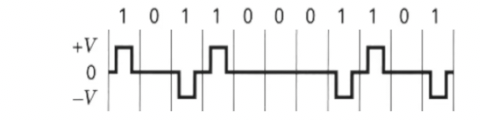
\includegraphics[width=0.6\textwidth]{../assets/ami.png}

\subsection{Bifase}

Aqui que a imaginação precisa ser um pouco maior, os níveis deixaram de ser tão óbvios, não é mais zero no meio de uma transição ou uma transição instantânea como no NRZ
é o tipo da transição, se sobe ou desce, é difícil visualizar isso então deixe eu fornecer uma maneira de pensar a respeito da distinção:
\\
\\
\textbf{Se for transição de subida
	imagine que é equivalente a jogar a parte antes do meio da transição para cima efetivamente parecendo com o NRZ-L para nível lógico 1 e se for descida repitir o processo obtendo
	o mapeamento no NRZ para nível lógico 0, conclusão, segundo essa lógica o bit 0 do NRZ seria mapeado no bit 1 do bifase e o contrário para o bit 1 do NRZ}.
\\

\textit{OBS:note ainda que as transições intermediárias, ocorrem no meio da transição, são garantidas por esse esquema, mas a que ocorrem no final não}
\\

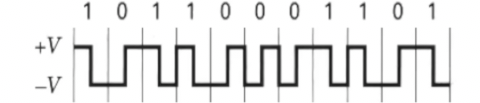
\includegraphics[width=0.6\textwidth]{../assets/bifasel.png}
\\\\
no caso o esquema acima se chama \textit{Manchester ou bifase-L}

Bem ainda existe o \textbf{Manchester Diferencial-M}, mas esse não será comentado nessas notas.

